\chapter{Introduction}
Since life's first beginnings, nature has been seeking optimal solutions to surviving in a constantly changing environment.
One key adaptation towards this goal, as evidenced by the ubiquity with which it is found throughout the tree of life, is the ability of an organism to anticipate daily changes to its environment.
Such rhythms are known as {\itshape circadian}, and are classified by a number of defining characteristics \cite{Dunlap2009}:

\begin{itemize}
  \item They are {\em endogenous}, meaning they continue to oscillate even when the organism is isolated from its environment

  \item They are temperature compensated, maintaining a consistent period for moderate changes in average temperature

  \item They are {\em entrainable}, meaning they can adjust their phase and period in response to a changing in environmental signal

  \item They oscillate with a roughly 24 hour period.
\end{itemize}

In this thesis, I apply techniques from systems biology in order to gain a more thorough understanding of how circadian rhythms control mammalian physiology, and how these rhythms might be altered through pharmacological therapies. % Really for abstract
Systems biology is a multidisciplinary field, drawing from biology, mathematics, and computer science. 
In this chapter, I first provide a background on the biology of circadian rhythms, followed by an introduction to the mathematical techniques which have been used to study them. 
I also discuss some computational considerations in the estimation of model parameters.

\section{Biological background}

\subsection{Dynamics of gene expression}

In the central dogma of molecular biology, genetic information is passed from DNA to mRNA to protein. 
While each cell in a multi-celled organism contains nearly identical DNA, the rate with which different genes are expressed results in substantial differences in cell type and function. 
These differences are the result of complex gene transcription networks, in which the production of some proteins - known as transcription factors - activate or repress the production of other genes. 
Similar to electrical circuits, network motifs such as positive and negative feedback arise from the interconnection of transcription factors.

Gene regulatory networks are essential to biological function. 
Cells maintain energy homeostasis by carefully balancing the flux of metabolites into energy storage and energy production pathways. 
These reactions are catalyzed by numerous enzymes, the activities of which must fluctuate to ensure the proper allocation of resources within a cell.
Enzyme production, degradation, and activation are controlled by transcription factors, and thus environmental conditions can be processed by complex network interactions to regulate metabolic function.
Circadian rhythms play a major role in the regulation of metabolic cycles, as periodic shifts in energy availability require a similar periodic shifts in gene transcription.

\subsection{Evolutionary history}

By looking at the evolutionary history of circadian rhythms, Edgar and colleges \cite{Edgar2012} demonstrated that cellular timekeeping may have began as a response to the Great Oxidation Event occurring $\approx 2.5$ billion years ago. 
Due to increased oxygen levels, the generation of reactive oxygen species in the cell can lead to oxidation of key biomolecules, prompting cells to express scavenging mechanisms during times of high UV light exposure. 
Over time, these pathways coupled to transcription-translation feedback loops in individual organisms, giving rise to a diverse set of circadian regulatory pathways (\fref{fig:edgarros}, from \cite{Edgar2012}). 

\begin{figure}[tbp]
  \centering
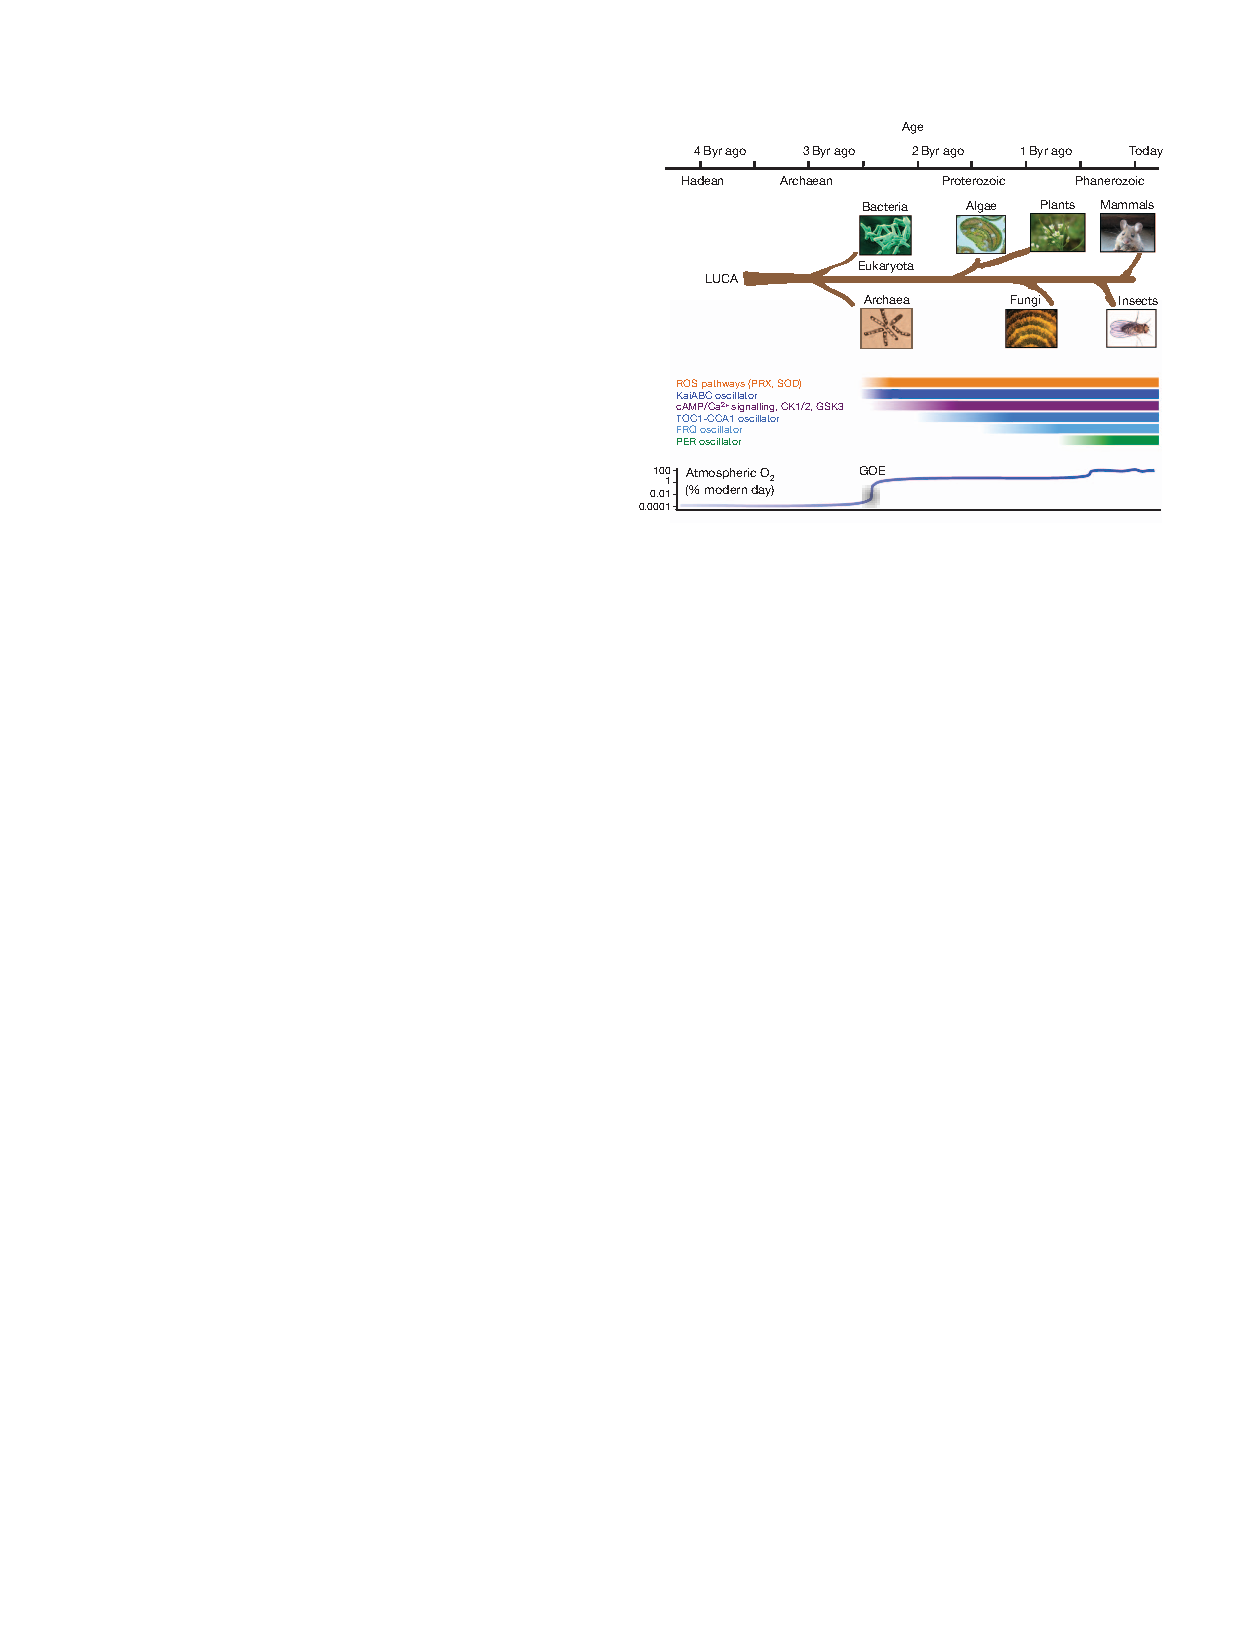
\includegraphics[width=0.8\textwidth]{chap1/figures/edgar_ros.pdf}
\titlecaption{Reactive oxygen species are conserved markers of circadian rhythms}{A timeline of the appearance of the main circadian feedback loops demonstrates that the rhythmic protection against light-mediated oxidation is a conserved rhythm across many evolutionary trees. Figure taken from \cite{Edgar2012}.}
  \label{fig:edgarros}
\end{figure}

\subsection{Circadian rhythms in mammals}

\subsubsection{Tissue-level clocks}

In mammals, circadian rhythms are organized in a hierarchical structure, in which inputs from the environment are processed separately by different tissue-level clocks (\fref{fig:feedforward}). 
Light, the primary entraining factor, is directed towards the suprachiasmatic nucleus (SCN), a tissue in the brain that serves as the body's master pacemaker \cite{Ralph1990}. 
In the SCN, approximately $20,000$ cells communicate via intercellular coupling to determine a precise internal time, which coordinates rhythms in locomotor activity \cite{Aton2005}.

\begin{figure}[tbp]
  \centering
  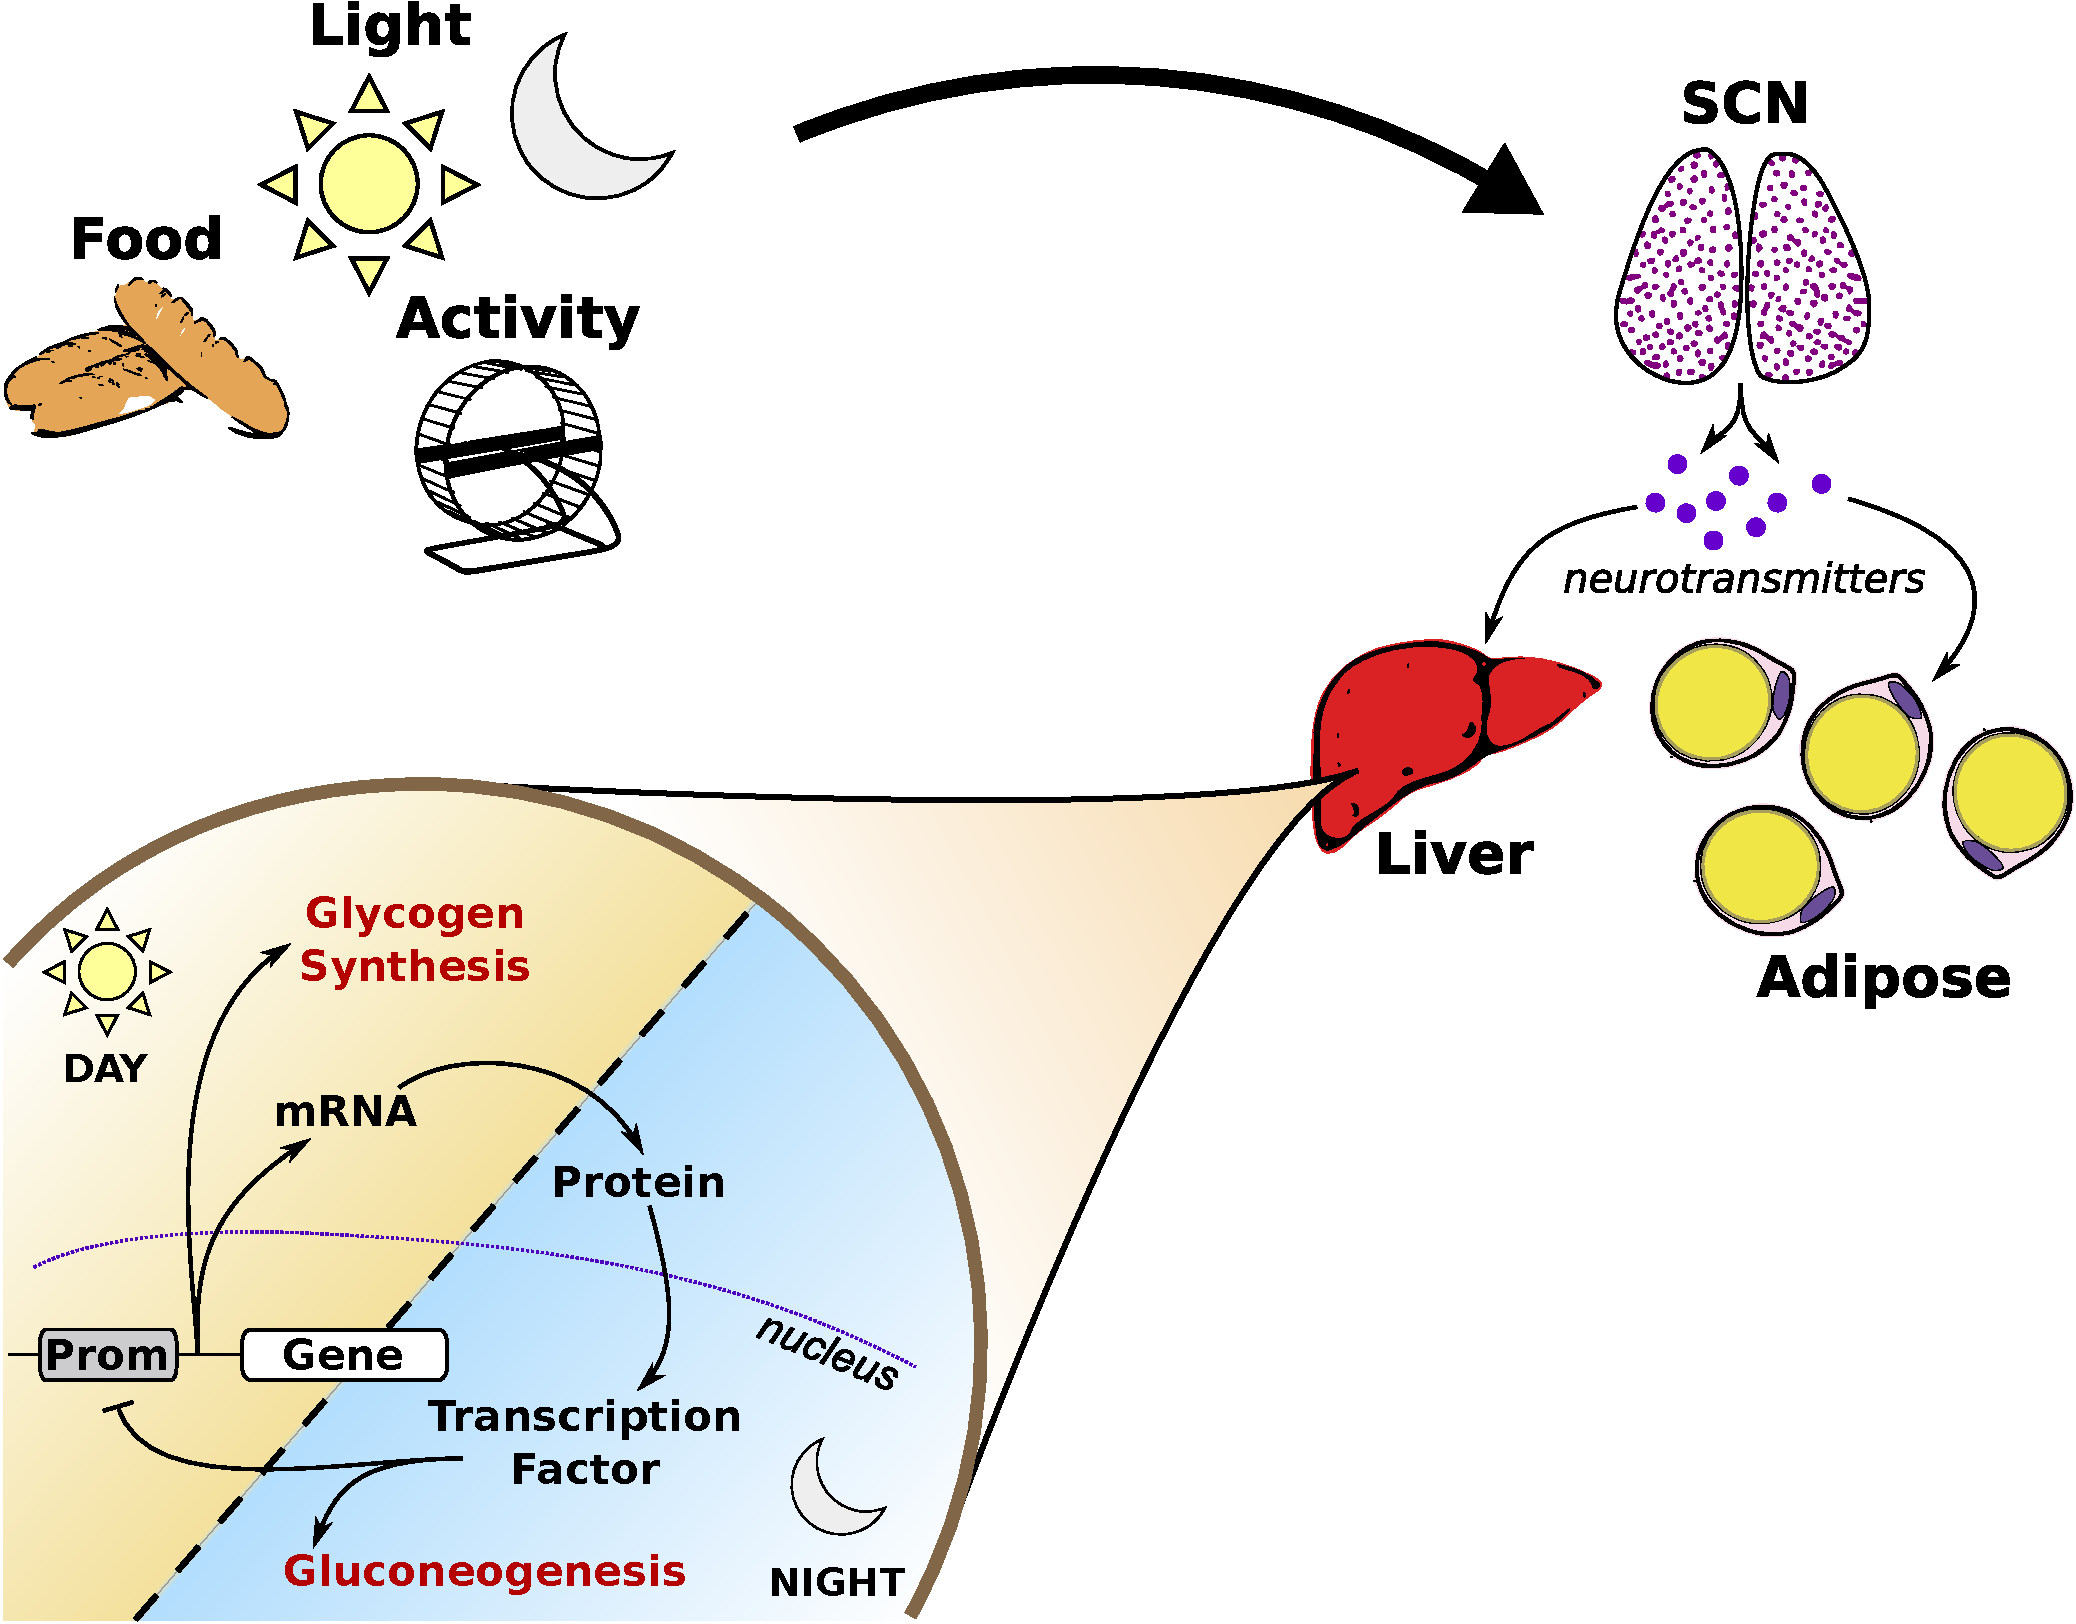
\includegraphics[width=\textwidth]{chap1/figures/timescale_separation.pdf}
  \titlecaption{A biological feed forward controller}{Circadian rhythms are organized in a heirarchical fashion, in which inputs from the environment are processed by different tissue-level clocks. At the single-cell level, rhythms are generated via a time-delayed transcription-translation negative feedback loop. Environmental inputs are used to predict upcoming environmental conditions by speeding or slowing the oscillatory cycle, matching the body's internal phase with the external environment.}
  \label{fig:feedforward}
\end{figure}

Peripheral tissues are responsible for responding to changes daily changes in food intake \cite{Bass2010}. 
Liver and adipose tissue, for instance, maintain robust circadian oscillations \cite{Yoo2004}, which respond mainly to temperature and food resetting cues \cite{Yamazaki2000a}.
Such clocks are important to maintaining metabolic health, as knockout experiments demonstrate that compromised circadian in peripheral tissues leads to many disorders, including diabetes and obesity \cite{Marcheva2010, Shi2013}.
Additionally, feeding cycles have been shown to have a profound impact on  circadian oscillations in peripheral tissues. High-fat or out of phase feeding leads to a reprogramming of oscillatory genes and metabolites 
\cite{Kohsaka2007, Hatori2012}, often leading to metabolic disease.

\subsubsection{Circadian oscillations at the single-cell level}
Circadian rhythms are generated at the single-cell level through genetic regulatory networks with inherent time-delayed negative feedback. 
Transcription factors CLOCK and BMAL1, peaking in the early night, activate expression of EBOX genes period ({\itshape Per1} and {\itshape Per2}) and cryptochrome ({\itshape Cry1} and {\itshape Cry2}). 
{\itshape Per} and {\itshape Cry} protein products, PER and CRY, peaking during the early day, form a heterodimeric complex to cross the nuclear membrane \cite{Ko2006}. 
However, since PER is present in the cytoplasm much lower quantities than CRY, it is stochiometrically-limiting for nuclear entry \cite{Lee2001}. 
Once inside the nucleus, the PER-CRY complex dissociates, and CRY represses CLOCK-BMAL1 mediated activation of EBOX genes, leading to rhythmic gene expression.
Several time delays contribute to the 24 hour oscillatory period, highlighted in \fref{fig:maindelays}.

\begin{figure}[tbp]
  \centering
  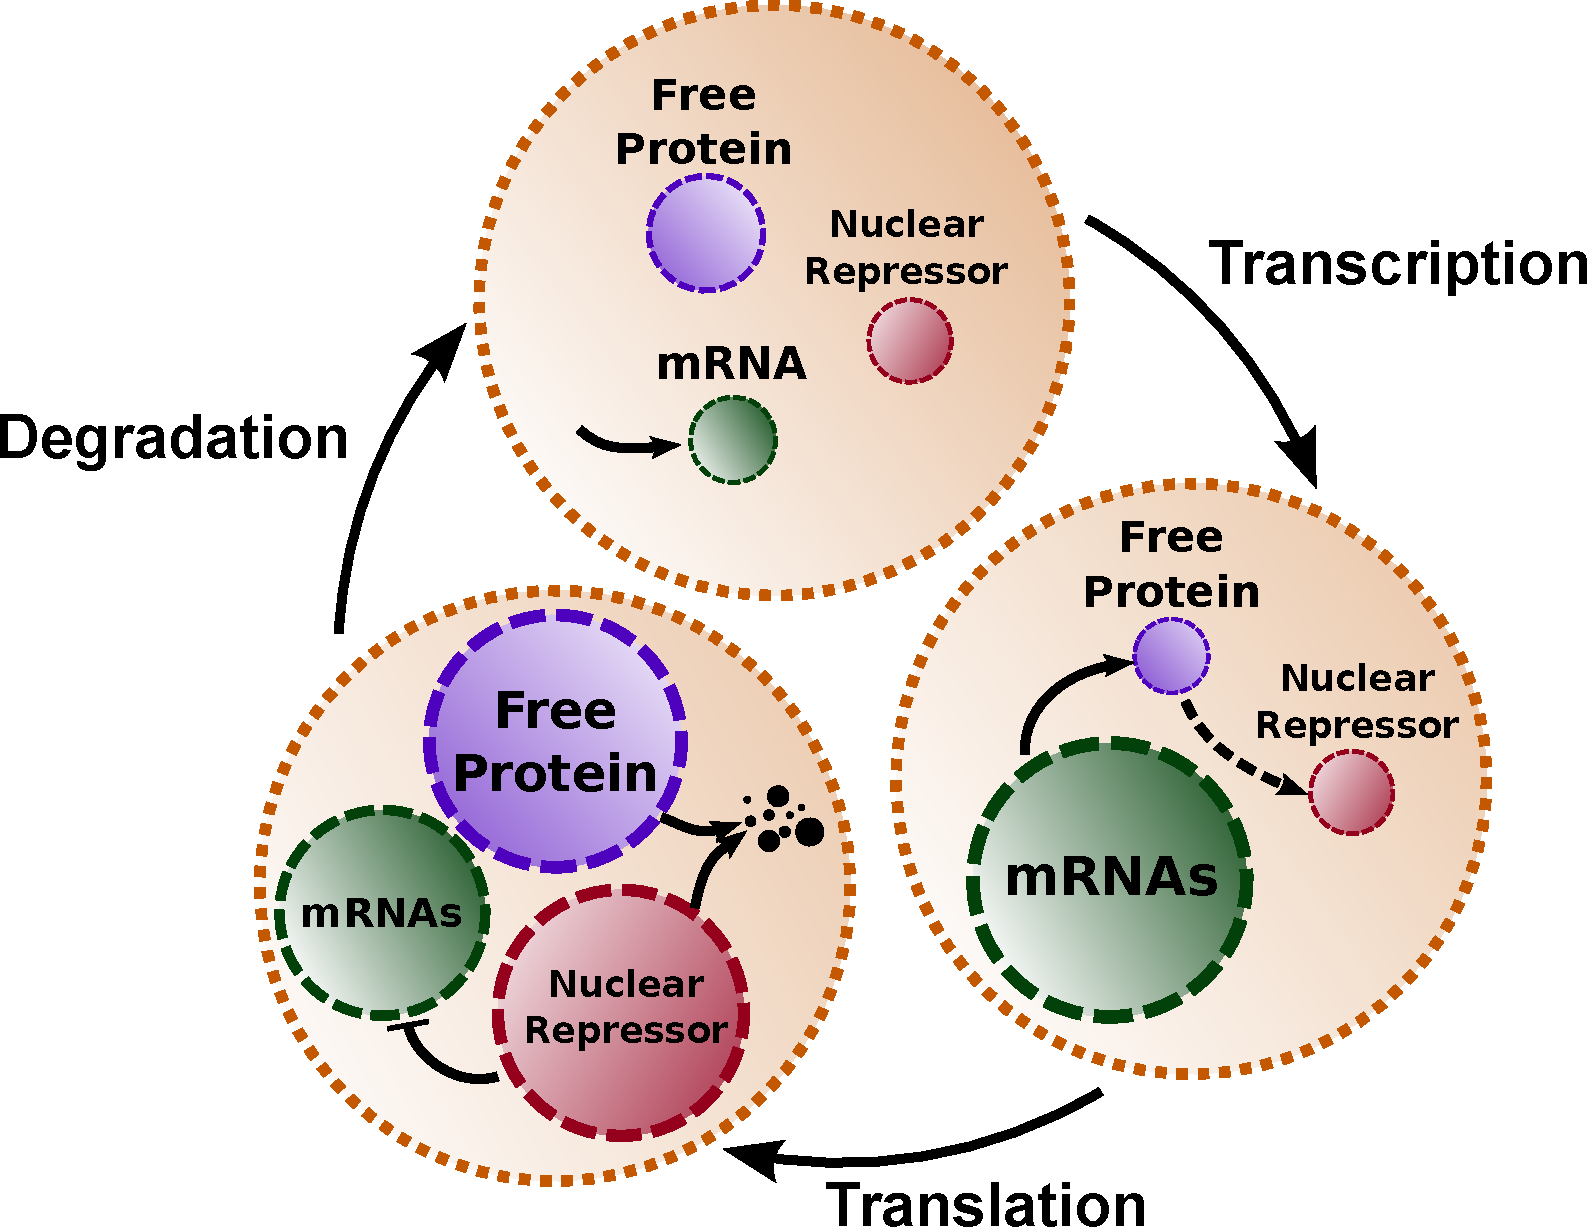
\includegraphics[width=0.7\textwidth]{chap1/figures/maindelays.pdf}
  \titlecaption{Key time delays}{Negative feedback may give rise to sustained oscillations in the presence of time delays. In the circadian system, these time delays are transcription, translation, and protein degradation. Each of these rates is a function of the external environment, resulting in entrainable oscillations.}
  \label{fig:maindelays}
\end{figure}

Additional components, namely the ROR and REV-ERB families of genes, add a layer of positive feedback to the clock regulatory loop.
This addition results in more reliable clock oscillations, as the bistability induced by the positive feedback stabilizes the negative-feedback induced oscillations \cite{Ananthasubramaniam2014a}.
A schematic of the core feedback in mammalian circadian rhythms is shown in \fref{fig:coreloop}.

\begin{figure}[tbp]
  \centering
  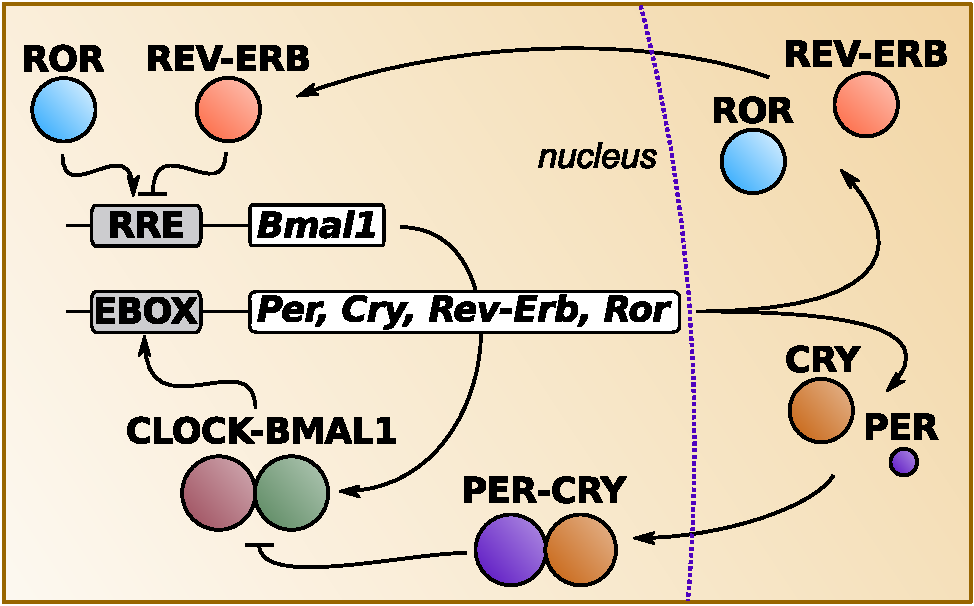
\includegraphics[width=0.7\textwidth]{chap1/figures/coreloop.pdf}
  \titlecaption{Core components of the mammalian circadian feedback loop}{The mammalian feedback loop is comprised of interlocking positive and negative feedback loops.}
  \label{fig:coreloop}
\end{figure}

\subsection{Experimental techniques}

While the focus of this thesis is primarily computational, I present a brief overview of the relevant experimental methods for studying circadian rhythms.
Most classical experiments determined the roles and importance of circadian genes using activity data of mouse knockouts \cite{Vitaterna1994}.
For instance, the period-determining effect of CRY1 and CRY2 were found by analyzing wheel-running behavior of mice in plots known as actograms \cite{VanderHorst1999}, as shown in \fref{fig:vanderhorst}.

\begin{figure}[tbp]
  \centering
  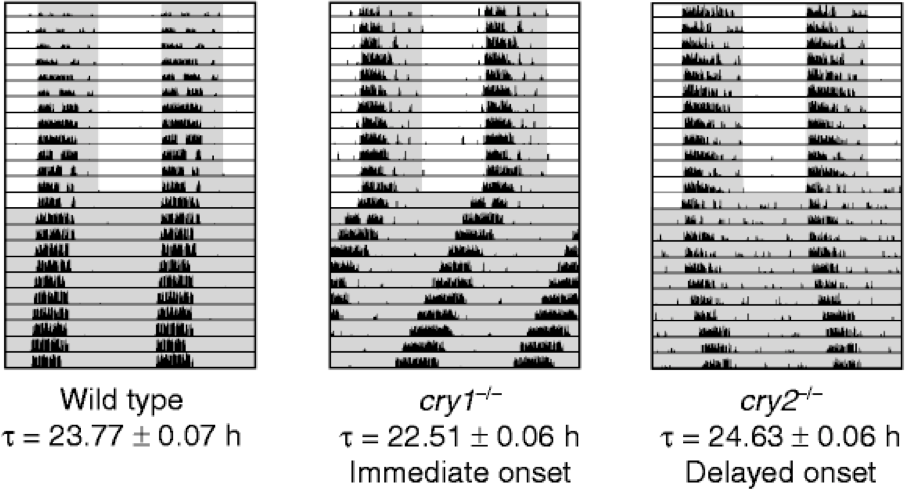
\includegraphics[width=0.7\textwidth]{chap1/figures/vanderhorst.png}
  \titlecaption{Period effects of CRY knockouts}{Actograms plot the intensity of mouse wheel-running activity on a 24 hr scale. After the mice are transferred to constant darkness, the free-running period can be inferred by fitting a line to the offset in activity onset each day. Figure taken from \cite{VanderHorst1999}.}
  \label{fig:vanderhorst}
\end{figure}

While activity-level knockout data is still used to characterize the effects of circadian perturbations, such methods are costly to implement and not amenable to high-throughput experimentation.
The development of luciferase reporter cell lines has rapidly changed the way circadian genes are screened \cite{Yoo2004}.
In reporter cells, the coupling of a luciferase protein to a core-clock gene allows the phase of rhythms to be determined by measuring the luminescence output from cultured cells, as shown in \fref{fig:chidalumin}.
Such systems have allowed the development of high-throughput methods for studying how siRNA \cite{Zhang2009} and small molecules \cite{Hirota2008} affect circadian parameters.

\begin{figure}[tbp]
  \centering
  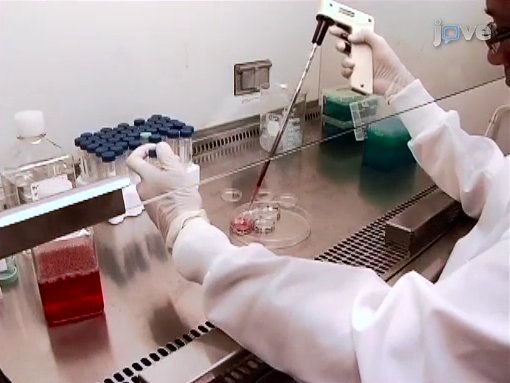
\includegraphics[width=0.45\textwidth]{chap1/figures/cells.png}
  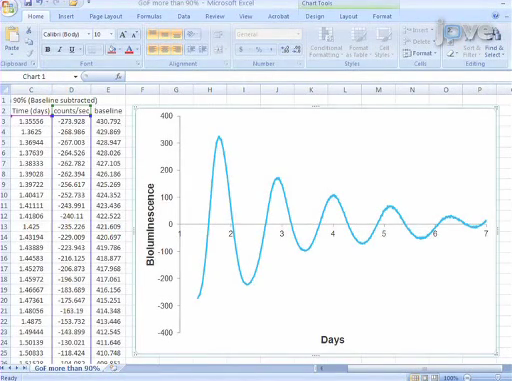
\includegraphics[width=0.45\textwidth]{chap1/figures/data.png}
  \titlecaption{Monitoring circadian parameters with bioluminescence reporter cell lines}{Cultured reporter cells allow parameters such as amplitude, period, and decay rate to be easily quantified. Image stills from \cite{Ramanathan2012}.}
  \label{fig:chidalumin}
\end{figure}

\section{Mathematical modeling}

Circadian rhythms, due to their dynamic nature, have long been a subject of mathematical inquiry \cite{Winfree2001}. In this section, I review some of the methods previously applied to understanding circadian rhythms.

\subsection{Introduction to modeling gene regulation}

Gene regulatory networks are typically modeled as dynamic systems, in which rates of production and degradation of each species is explicitly considered.
In \fref{fig:sysbiointro}, an example gene regulatory network is shown, in which a transcription factor activates the production of Gene 1. 
The genes mRNA is then translated to produce a protein product, which may or may not undergo posttranslational modifications or subcellular transport. 
The completed protein then modulates the production of a second mRNA, for Gene 2.
In this example, the production and degradation rates of the mRNA and each protein state would be explicitly modeled.

\begin{figure}[tbp]
  \centering
  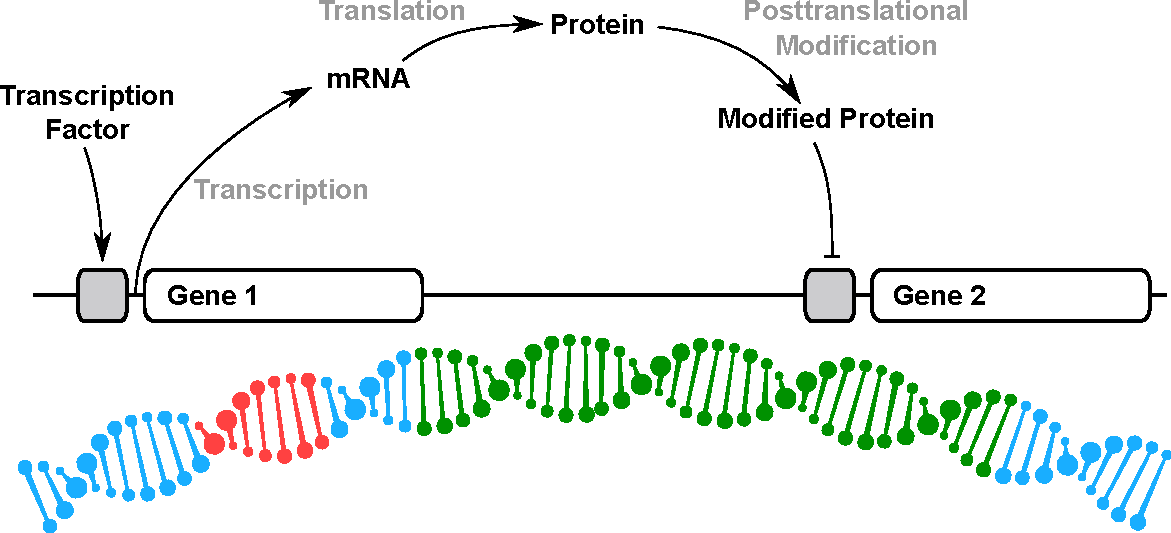
\includegraphics[width=\textwidth, clip=True, trim=0 100 0 0]{chap1/figures/sysbio_intro.pdf}
  \titlecaption{Gene regulatory networks can be modeled as dynamic systems}{Transcription, translation, degradation steps are treated as chemical reactions, in which the reaction rate depends only on the current concentration of other species and various kinetic parameters.}
  \label{fig:sysbiointro}
\end{figure}

If the values of the kinetic parameters (i.e., transcription rate) were known, the model could subsequently be simulated by casting the equations as either a system of ordinary differential equations (as in \fref{sec:odes}), or by using a chemical master equations (as in \fref{sec:stoch}). Resulting trajectories would resemble those shown in \fref{fig:extrajs}.

\begin{figure}[tbp]
  \centering
  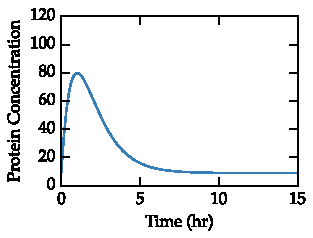
\includegraphics[width=0.475\textwidth]{chap1/figures/sysbio_trajs1.pdf}
  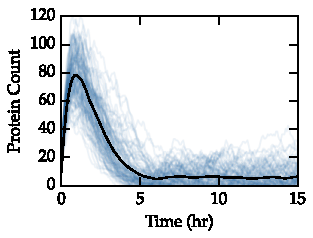
\includegraphics[width=0.475\textwidth]{chap1/figures/sysbio_trajs2.pdf}
  \titlecaption{Simulated time-dependent concentration trajectories}{(Left) Deterministic simulations of the dynamic system result in expected values for each state variable over time. (Right) Stochastic simulations account for the intrinsic noise present due to the low molecule counts of each reactant. From these simulations, more realistic noise estimates can be obtained at the expense of a greater computational complexity.}
  \label{fig:extrajs}
\end{figure}

\subsection{Ordinary differential equations}\label{sec:odes}

Ordinary differential equation (ODE) models take the general form
\begin{equation}
  \frac{dx}{dt} = f(x(t), p),
  \label{eq:odefn}
\end{equation}
in which $x(t)$ represents the concentrations of the state variables, such as mRNA and protein concentrations, $f$ contains information on the production, degradation, and reactivity of the states, and $p$ are the kinetic parameters which govern reaction kinetics.
Limit cycle models are ODE models in which the solution approaches a steady state oscillatory trajectory, satisfying the equation:
\begin{equation}
  \lim_{t \to \infty} \left[ x(t + T) - x(t) \right] = 0.
  \label{eq:limit5}
\end{equation}
The period is the smallest $T > 0$ for which \fref{eq:limit5} holds. 
An example periodic limit cycle is shown in \fref{fig:statespace}, which plots the deterministic solution to \fref{mod:novak}.

\begin{figure}[tbp]
  \centering
  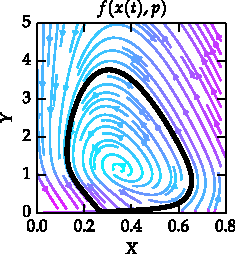
\includegraphics[width=0.45\textwidth]{chap1/figures/state_space.pdf}
  \titlecaption{State-space representation of a deterministic limit cycle}{A two-dimensional oscillator, \fref{mod:novak}, allows the system dynamics to be easily plotted. The steady state limit cycle, $x^\gamma(\theta)$, is shown in dark black. Points which lie off the limit cycle will eventually converge, following the vector field arrows. Colors represent the speed with which the solution will travel, with warmer colors indicating faster speeds.}
  \label{fig:statespace}
\end{figure}


The points on the stable limit cycle are denoted by $x^\gamma(\theta)$ with each point assigned to a value of a phase variable $\theta \in [0, 2\pi)$.
For convenience, time in \fref{eq:odefn} can be rescaled such that the period is $2\pi$:
\begin{equation}
  \tilde{t} = \frac{2\pi}{T}t; \quad \tilde{f} = \frac{T}{2\pi}\;f; \quad \frac{dx}{d\tilde{t}} = \tilde{f}(x(\tilde{t}), p).
  \label{eq:that}
\end{equation}
The phase variable $\theta$ is therefore defined on the limit cycle as $\theta = \tilde{t}\mod 2\pi$, with $\theta = 0$ assigned to a unique and identifiable point. An example mapping of the phase variable $\theta$ for \fref{mod:novak} is shown \fref{fig:phasedef}

\begin{figure}[tbp]
  \centering
  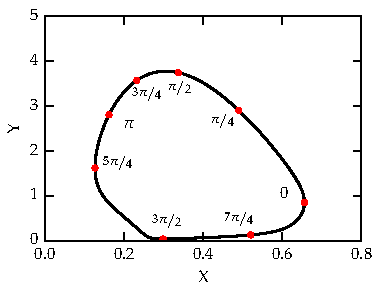
\includegraphics[width=0.5\textwidth]{chap1/figures/phase_def.pdf}
  \titlecaption{Definition of the phase variable}{A phase variable $\theta$ maps each point on the limit cycle, $x^\gamma(t)$, to a unique value of the phase. Because the definition of $\theta$ depends on time, the distance in state-space between each phase point is not equal.}
  \label{fig:phasedef}
\end{figure}


\subsection{ODE sensitivity analysis}

When analyzing ODE models, it is often important to know how the solution varies with respect to initial values or parameters. 
The sensitivity matrix is defined as
\begin{equation}
  S(t) = \frac{dx(t)}{dx(0)} = \lim_{\Delta x(0) \to 0}\frac{\Delta x(t)}{\Delta x(0)}.
  \label{eq:senslimit}
\end{equation}
While it is possible to obtain estimates of these derivatives through finite difference methods, more accurate and less computationally intensive representations can be obtained by integrating these sensitivities along with the original ODE system \cite{Dickinson1976}. 
The differential equation for the sensitivity system is shown in equation~\ref{eq:senslimit}. 
\begin{equation}
  \frac{d}{dt} S(t)  = \frac{df(x(t),p)}{dx}\; S(t)
  \label{eq:odesens}
\end{equation}
Since the jacobian matrix $\frac{\partial f}{\partial y}$ is the same as that of the original ODE system, efficient implementations of the following ODEs have been developed \cite{Feehery1997}.

\subsubsection{Period sensitivity}

An extension of sensitivity analysis for limit-cycle specific models raises additional complications. 
For instance, finding the derivative of the period with respect to parameter values requires a clever decomposition of the sensitivity matrices \cite{Kramer1984}. 
Period sensitivities, $\frac{\partial T}{\partial p}$, can be obtained directly from sensitivities integrated for one pass of the limit cycle (derived in \cite{Wilkins2009}) through a linear solve:
\begin{equation}
  \left[\begin{array}{cc}
      \mathbf{M} - \mathbf{I} & \dot{x}(T) \\
      \frac{\partial f_0}{\partial x}(x(0)) & 0
  \end{array}\right]
  \left[\begin{array}{c}
      \vdots \\ \frac{\partial T}{\partial p}
  \end{array}\right] =
  \left[\begin{array}{c}
      -\mathbf{S}(T) \\ -\frac{\partial {\bm f}}{\partial p}(x(0))
  \end{array}\right]
\end{equation}
in which $\mathbf{M}$ is the Monodromy matrix, $\mathbf{I}$ is the identity matrix, and the unknown vector contains the relevant period sensitivities.

Since parameter values often span several orders of magnitude, an often more useful measure is the relative period sensitivity, which is independent of the magnitude of the period or parameter value.
\begin{equation}
  \frac{\partial \ln T}{\partial \ln p} = \frac{p}{T}\frac{\partial T}{\partial p} = \frac{\partial T}{T} \left/ \frac{\partial p}{p} \right.
\end{equation}
Thus, a relative period sensitivity of 1 indicates that a 1\% increase in the parameter value will result in a 1\% increase in the period.

\subsubsection{Phase sensitivity}

Additionally, perturbations to state variables away from a limit cycle ultimately return, but with in a change of phase.
The definition of phase can be extended to points outside the limit cycle, $x_0 \not\in x^\gamma(\theta)$, by defining the phase of any point, $\Theta(x_0)$, as the initial phase of a point on the limit cycle to which $x_0$ will ultimately converge:
\begin{equation}
  \Theta(x_0) = \arg\min_\theta \lim_{t \to \infty} \lVert x(t)
  - x^\gamma(\theta + t)\rVert
  \label{eq:extendedphase2}
\end{equation}
A phase response curve (PRC), which maps the change in phase resulting from the same
perturbation applied at every phase, can therefore be found by calculating $
\Delta\theta \coloneqq \Theta(x^\gamma(\theta_0) + \Delta x(0)) - \theta_0$ for each
$\theta_0$. Infinitesimal PRCs, the derivative of the phase
change with respect to the perturbation, are defined for state and
parameter-impulse perturbations as \cite{Taylor2008a}:
\begin{align}
  \frac{d\theta}{dx} &\coloneqq \lim_{\Delta x(0) \to 0} \frac{\Delta\theta}{\Delta
  x(0)} \label{eq:sPRC}\\
  \frac{d}{d\hat{t}}\frac{d\theta}{dp} &\coloneqq \lim_{d,\; \Delta p \to 0}
  \frac{\Delta\theta}{d \; \Delta p}
  \label{eq:PRC}
\end{align}
Methods for efficiently calculating these quantities using ODE sensitivity
analysis have been developed \cite{Taylor2008a}, with the important result
that, in the limit as $d, \Delta p \to 0$, 
\begin{equation}
  \frac{d}{d\hat{t}}\frac{d\theta}{dp} = \frac{d\theta}{dx}\frac{d\hat{f}}{dp} 
  \label{eq:pPRCequiv}
\end{equation}

\subsection{Stochastic methods}\label{sec:stoch}

In modeling a system of chemical reactions using ODE methods, the assumption is made that the concentration of reacting species can take any continuous value. 
While this assumption is often appropriate for reactions in large, well-mixed vessels, it is often not the case in reactions that take place in the cell.
In mammalian cells, the median number of mRNA transcripts per cell is $17$, while the median number of protein copies is $50,000$ \cite{Schwanhausser2011}.
As a result, low concentrations of state variables are often best represented by discrete steps, in which the probabilistic nature of reaction events plays a large role in determining the system dynamics.

Stochastic systems are specified by a state vector of discrete populations $x = \{x_1, \ldots, x_N\}$ and reaction vector $R = \{R_1, \ldots, R_M\}$. 
For each of $M$ reactions, a stoichiometric vector $v_i$ describes the states which are produced and consumed by each reaction, and a reaction propensity function $a_i$ describes the likelihood of the reaction in for time step \cite{Gillespie1977}.
Together, these equations form the chemical master equation, a Markov (memoryless) process which can be efficiently simulated using a variety of algorithms \cite{Sanft2011}.



